\capitulo{4}{Técnicas y herramientas}
\begin{comment}
\section{Stream Processing Framework}

Stream processing es una tecnología que procesa los datos de forma continua y secuencial, para realizar esta tarea se utilizan flujos de datos infinitos y sin límites de tiempo. Son extremadamente útiles a la hora de monitorizar sistemas, redes, aplicaciones, dispositivos, etc... 

algunas de las alternativas más populares que he considerado son las siguientes:

\subsection{Apache Kafka}

Apache Kafka es un sistema de intermediación de mensajes que responde al patrón "Publish/Subscribe Messaging" que se utiliza para la comunicación entre aplicaciones. Entre sus principales características se encuentran que es un sistema escalable y persistente, con gran tolerancia a fallos y gran velocidad tanto de escritura cómo de lectura.

Para transmitir estos datos Kafka crea \textit{Topics}, flujos de datos que a su vez se dividen en particiones, cada mensaje se almacena en una de estas particiones.

Debido a su popularidad es una herramienta bien documentada \cite{documentacion:kafka} tanto por la propia compañía cómo los usuarios. \cite{pagina:kafka}

\subsection{Apache Airflow}
Apache Airflow es una plataforma open-source que nos permite automatizar tareas con la ayuda de scripts y mediante el uso de un planificador para llevar a cabo numerosas tareas. Permite la utilización de DAGs (Grafo acíclico dirigido) y crear pipelines dinámicos, mediante Python. 

Apache Airflow tiene una curva de aprendizaje elevada y puede resultar complicado para los usuarios\cite{pagina:HEVO}

\subsection{Apache Samza}
Es un procesador de flujo a tiempo real, usa Apache Kafka para la mensajería y Apache Hadoop YARN para tolerancia a fallos, seguridad, independencia de procesos y gestión de recursos para su utilización es necesario Hadoop. Samza utiliza streams inmutables e implementa el procesamiento de flujo sin y con estado. \cite{pagina:Samza}

\subsection{Apache Flume}

Apache Flume es un servicio distribuido capaz de mover grandes cantidades de datos y logs, este forma parte del ecosistema de Hadoop. Su arquitectura es tanto flexible cómo sencilla. aunque presenta cierta dificultad a la hora de escalar. Está basado en flujo de datos en Streaming permitiendo múltiples flujos.\cite{pagina:Flume}
\end{comment}
\section{Visualización y análisis de datos}

Para monitorizar nuestros datos debemos hacer uso de herramientas de Network monitoring que nos permita detectar fallos y anomalías en los datos así cómo alertarnos si alguno de los datos monitorizados pasa por debajo de un umbral.

\subsection{PRTG Network Monitor}

PRTG Network Monitor es una herramienta de monitorización desarrollada por Paessler, que permite supervisar y monitorizar datos de sensores, la versión gratuita está limitada a 100 sensores, una de las ventajas de PRTG es la cantidad de variedad de sensores que existen de forma predefinida. Permite mostrar alertas al encontrar problemas o métricas inusuales.\cite{pagina:PRTG}

\subsection{ThingSpeak}

ThinkSpeak es una plataforma open source orientada al Internet de las Cosas (IOT) que permite recoger, almacenar datos de sensores en la nube usando el protocolo HTTP y visualizar los datos. También permite realizar análisis de los datos usando MATLAB. 

ThingSpeak consta de aplicaciones complementarias con diversas funcionalidades. \cite{pagina:ThingSpeak}

\subsection{Grafana}

Grafana permite visualizar y representar métricas de datos sin importar donde estén almacenados, la visualización es rápida y flexible con multitud de opciones. En Grafana se pueden definir alertas sobre las métricas que se desee y manda notificaciones de estas, también cuenta con cientos de plugins oficiales. 

Contiene una opción de pago en la que ellos proporcionan el servidor y otro completamente gratuita en la que permite ejecutarlo en cualquiera de los sistemas operativos principales.\cite{pagina:Grafana}

\subsection{Splunk}
Splunk es una plataforma que permite monitorizar, buscar y analizar datos en tiempo real, esta herramienta consta de cientos de aplicaciones y es compatible con casi cualquier formato de logs. Splunk es gratis con un volumen de datos diarios de menos de 500 MB. \cite{pagina:Splunk}

Uno de sus atractivos es que consta de una herramienta machine learning que aprende de tus datos detectando anomalías y prediciéndolas.

\subsection{Elección final}
Debido a que el cliente que va a facilitar los datos de los sensores utiliza PRTG se he optado por esta opción.

\section{Motor de búsquedas}

\subsection{Algolia}
Algolia es un motor de búsqueda accesible vía API, la cual se puede integrar en web y aplicaciones móviles. Funciona exclusivamente con datos en formato JSON. Algolia posee una inteligencia artificial que aprende del usuario para mejorar su experiencia de uso. Consta de una versión gratuita, la cual tiene limitada el número de resultados de búsqueda.\cite{pagina:Algolia}

\subsection{Elasticsearch}
Elasticsearch es uno de los motores de búsqueda más valorados del mercado\cite{ranking:DB-Engines} , de código abierto que proporciona análisis y búsqueda de datos a tiempo real. Esta desarrollado en Java y sólo soporta JSON cómo tipos de respuesta.

Posee una arquitectura distribuida siendo la escalabilidad horizontal, una de sus ventajas es su rapidez a la hora de realizar búsquedas de textos complejos para facilitar esto funciona mediante índices invertidos.\cite{pagina:ElasticSearch}  

\subsection{Solr}
Apache Solr es un motor de búsqueda open source escrito en java con comandos escritos en HTTP y guarda los archivos utilizando XML. Esta optimizado para tráfico de altos volúmenes de datos y todo en tiempo real.\cite{pagina:Solr} 

\subsection{Elección final}

Debido a que el entorno de ElasticSearch facilita la ingesta de datos, almacenamiento y la posterior visualización de estos se ha elegido esa opción.

\section{Control de versiones}

Herramientas consideradas: GitHub y GitLab.

Para organizar el proyecto se ha elegido la plataforma de control de versiones de GitHub debido a ser el software de versiones Git más utilizado.

\section{Lenguajes de programación}

\subsection{Python}
Python es un lenguaje de programación multiplataforma y multiparagigma, soporta tanto programación orientación a objetos cómo programación imperativa. Es un lenguaje cuya sintaxis se centra en un código legible y sintaxis clara. \cite{pagina:Python_documentation}

\subsection{Bash}
GNU Bash es una interfaz de usuario de línea de comandos y un lenguaje de programación de scripting, se creó originalmente para el sistema operativo GNU. Actualmente disponible en la mayoría de distribuciones GNU/Lunux, Mac OS X y también tiene versiones para Windows 10 y Android.

\section{librerias Python}

\subsection{Scikit-learn}

Scikit-learn es un módulo de programación en python para machine learning, permite realizar algoritmos de clasificación, regresión, Análisis de grupos, Máquinas de vectores de soporte, Árboles de decisión, etc...

Scikit-learn trabaja a su vez con otras librerías cómo NumPy, SciPy, pandas, SymPy, Matplotlib, Ip[y].\cite{pagina:scikit-learn}

\subsection{scikit-multiflow}

Scikit-multiflow es una librería de machine learning para python dedicada a streaming data y multi-output learning que permite generar y evaluar data streams.\cite{skmultiflow}

\subsection{NumPy}
NumPy es una librería de Python especializada en el cálculo numérico y computación de datos. 

\subsection{Pandas}

Pandas es una librería open source de programación para Python y utilizando cómo extensión NumPy, se utiliza para análisis de datos, ofreciendo estructuras de datos y operaciones con tablas numéricas y series temporales.\cite{pagina:wiki_pandas}


\subsection{River}
River es una librería de maching learning en streaming para python, juntando las librerías creme y sckit-multiflow.

Es una librería reciente por lo que la documentación no está completa y aún no hay muchos proyectos que hayan utilizado la librería.\cite{pagina:River}

\section{Archivos de texto}
\subsection{JSON}
El formato de texto JSON (JavaScript Object Notation) se utiliza para el intercambio de datos. Resulta sencillo tanto de leerlo cómo de escribirlo para los humanos y sencillo de interpretarlo y generarlo para las máquinas.

El formato JSON es independiente del lenguaje JavaScript.

En este trabajo he decidido utilizar JSON para el intercambio de datos sobre otros formatos como CSV por su sencillez y su compatibilidad con PRTG y Elasticsearch.\cite{pagina:JSON}


\section{Sistemas Operativos}

\subsection{Windows 10}
Debido a que el cliente que va a facilitar los datos utiliza PRTG para monitorizar los sensores y este es exclusivo de Windows no se tiene más alternativa que utilizar este sistema operativo para albergar un servidor PRTG.

\subsection{Ubuntu Server 20.04.2}
Para albergar tanto Elasticsearch como el programa que conecte todos los sistemas se a escogido la última versión de ubuntu server debido a su ligera y por la facilidad que este tendría para implementarlo en un servidor real.

\section{IDEs}

\subsection{\LaTeX}
Herramientas consideradas: Overleaf y Textmaker

La herramienta que se ha decidido utilizar para redactar la memoria y los anexos de este proyecto ha sido Overleaf divido a que es un sencillo editor \LaTeX basado en la nube y no requiere de ninguna instalación previa.

\subsubsection{Vim}
Para la edición de archivos de texto en el servidor de Ubuntu se ha decidido utilizar vim debido a que es un editor que en los sistemas ubuntu ya viene preinstalado además de su gran versatilidad y ligereza.

\subsubsection{Jupyter Notebook}

Es una aplicación cliente-servidor que permite crear y compartir documentos web con formato JSON. Jupyter soporta los lenguajes de programación Julia, Python y R.

En este proyecto se utiliza para documentar las pruebas realizas.\cite{pagina:Jupyter}

\section{Virtualización}

\subsubsection{VirtualBox}
Para albergar las máquinas virtuales se ha utilizado VirtualBox debido a ser la herramienta open source más famosa de virtualización.

\begin{comment}

\section{Procesadores de lenguaje}
Herramientas consideradas: Flex, Bison, JavaCC

Debido a la baja complejidad y el poco uso que le iba a dar a esta herramienta he decidido utilizar Flex, un analizador de lenguaje open source.
\end{comment}

\section{Comunicación}
\subsection{Microsoft Teams}
Microsoft Teams es una plataforma de comunicación y colaboración para reuniones telemáticas.

\section{Cliente SSH}
\subsection{PuTTY}
PuTTY es un cliente SSH  y telnet con licencia libre.

Este software permite conectarse de forma remota a al Ubuntu server así cómo intercambiar ficheros entre el server y el host.

\section{ELK Stack}
ELK es la combinación de Elasticsearch, Logstash y Kibana.

\begin{figure}[h]
	\centering
	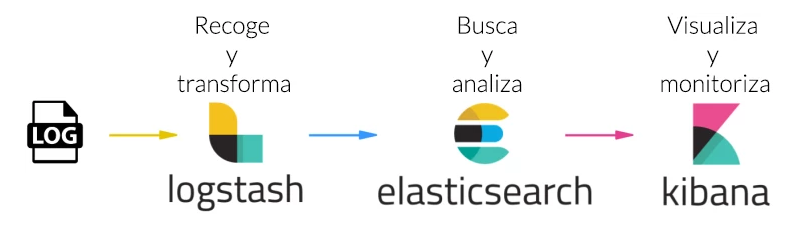
\includegraphics[width=1.1\textwidth]{img/img_resumen_ELK.png}
	\caption{ELK Stack}
	\label{img_resumen_ELK}
\end{figure}

\subsection{Elasticsearch}
Cómo se comentado con anterioridad en el apartado de motores de búsqueda Elasticsearch se encarga del almacenamiento de datos y aporta un potente motor de búsqueda.

\subsection{Logstash}
Logstash es un pipeline de procesamiento de datos capaz de ingresar datos de múltiples fuentes y enviarlos a una variedad de salidas, pero en el caso de nuestro programa será Elasticsearch.

\subsection{Kibana}
Kibana es una interfaz de usuario que permite la visualización de datos de Elasticsearch. Esta herramienta nos facilita la creación de histogramas, gráficos, mapas y demás formas gráficas de representación de los datos.